% TeX eps-loader file generated by McmcDiagnostics.m (Dynare).
% 02-May-2024 14:06:42
 
\begin{figure}[H]
\centering 
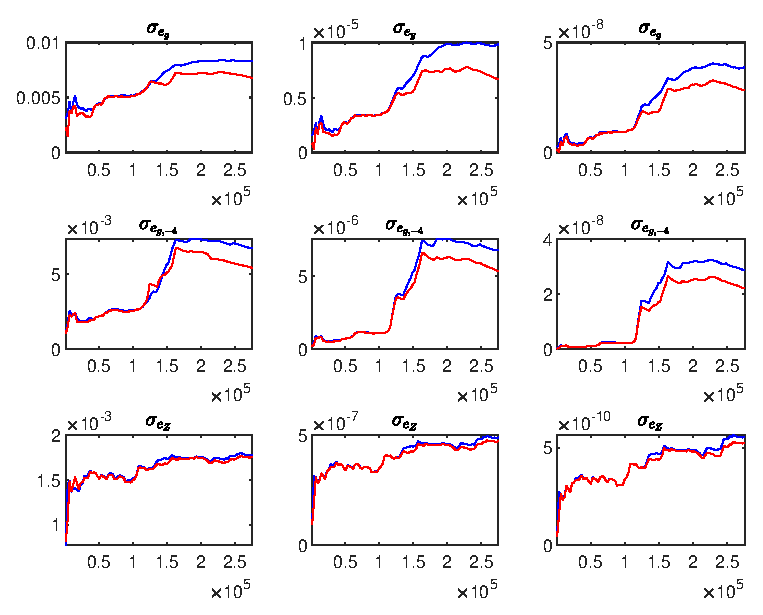
\includegraphics[width=0.80\textwidth]{BRS_sectoral_artificial_data/Output/BRS_sectoral_artificial_data_udiag1}
\caption{Univariate convergence diagnostics for the Metropolis-Hastings.
The first, second and third columns are respectively the criteria based on
the eighty percent interval, the second and third moments.}\label{Fig:UnivariateDiagnostics:1}
\end{figure}

\begin{figure}[H]
\centering 
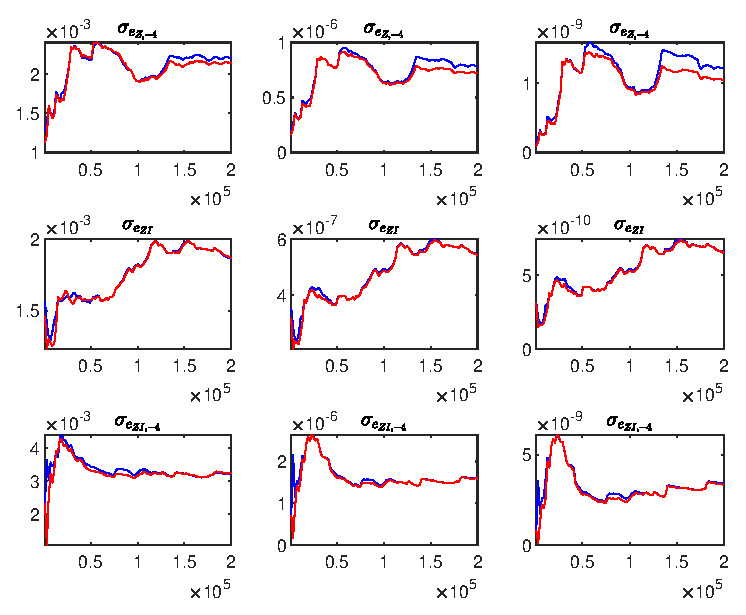
\includegraphics[width=0.80\textwidth]{BRS_sectoral_artificial_data/Output/BRS_sectoral_artificial_data_udiag2}
\caption{Univariate convergence diagnostics for the Metropolis-Hastings.
The first, second and third columns are respectively the criteria based on
the eighty percent interval, the second and third moments.}\label{Fig:UnivariateDiagnostics:2}
\end{figure}

\begin{figure}[H]
\centering 
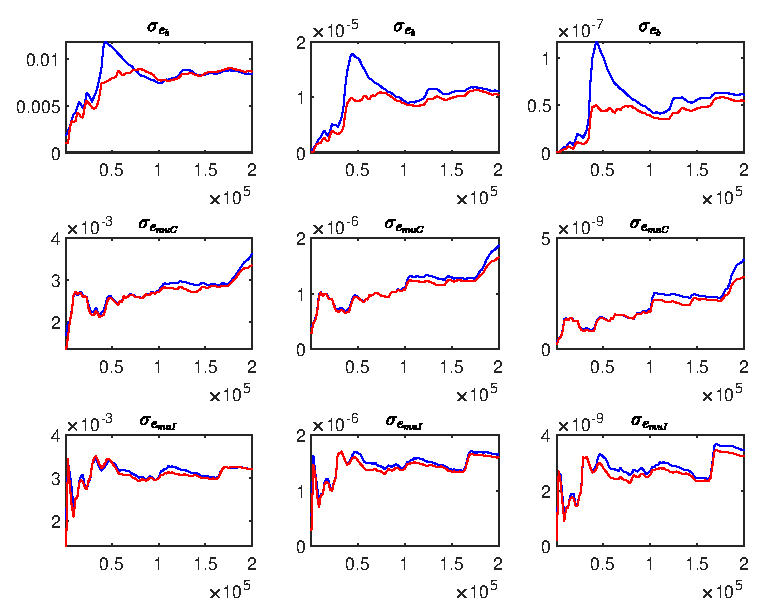
\includegraphics[width=0.80\textwidth]{BRS_sectoral_artificial_data/Output/BRS_sectoral_artificial_data_udiag3}
\caption{Univariate convergence diagnostics for the Metropolis-Hastings.
The first, second and third columns are respectively the criteria based on
the eighty percent interval, the second and third moments.}\label{Fig:UnivariateDiagnostics:3}
\end{figure}

\begin{figure}[H]
\centering 
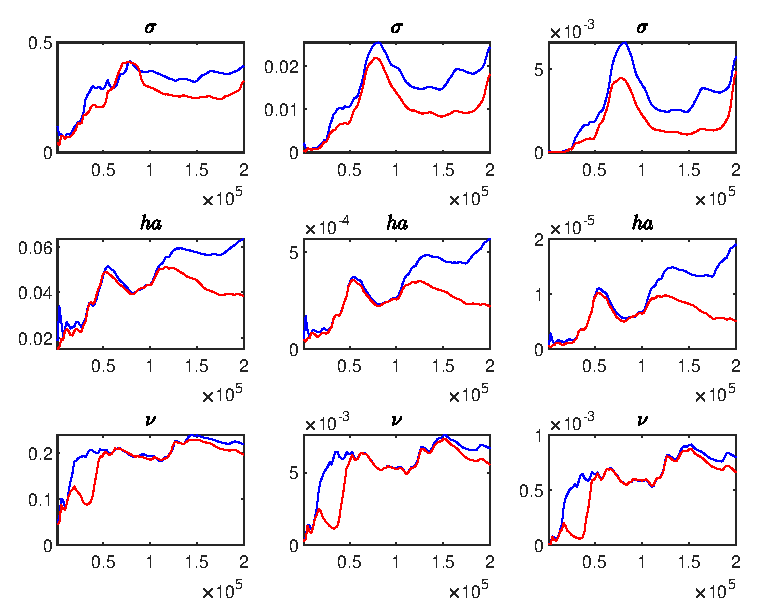
\includegraphics[width=0.80\textwidth]{BRS_sectoral_artificial_data/Output/BRS_sectoral_artificial_data_udiag4}
\caption{Univariate convergence diagnostics for the Metropolis-Hastings.
The first, second and third columns are respectively the criteria based on
the eighty percent interval, the second and third moments.}\label{Fig:UnivariateDiagnostics:4}
\end{figure}

\begin{figure}[H]
\centering 
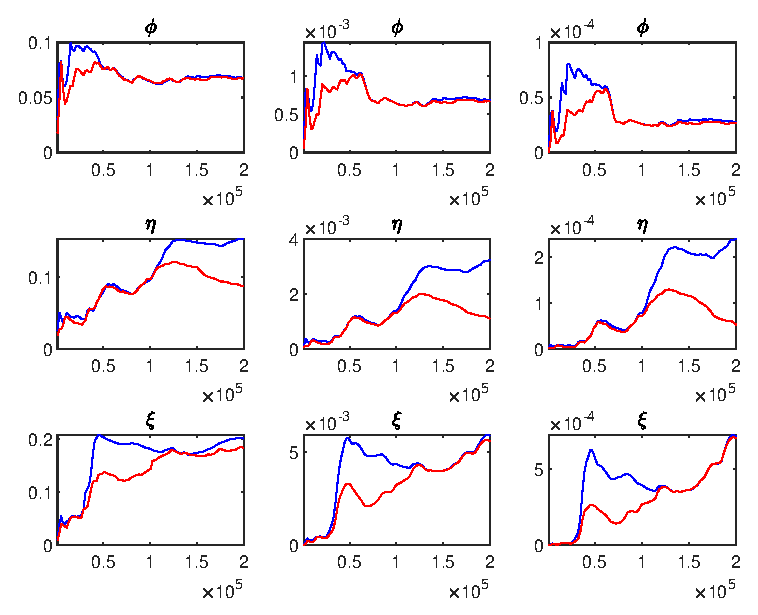
\includegraphics[width=0.80\textwidth]{BRS_sectoral_artificial_data/Output/BRS_sectoral_artificial_data_udiag5}
\caption{Univariate convergence diagnostics for the Metropolis-Hastings.
The first, second and third columns are respectively the criteria based on
the eighty percent interval, the second and third moments.}\label{Fig:UnivariateDiagnostics:5}
\end{figure}

\begin{figure}[H]
\centering 
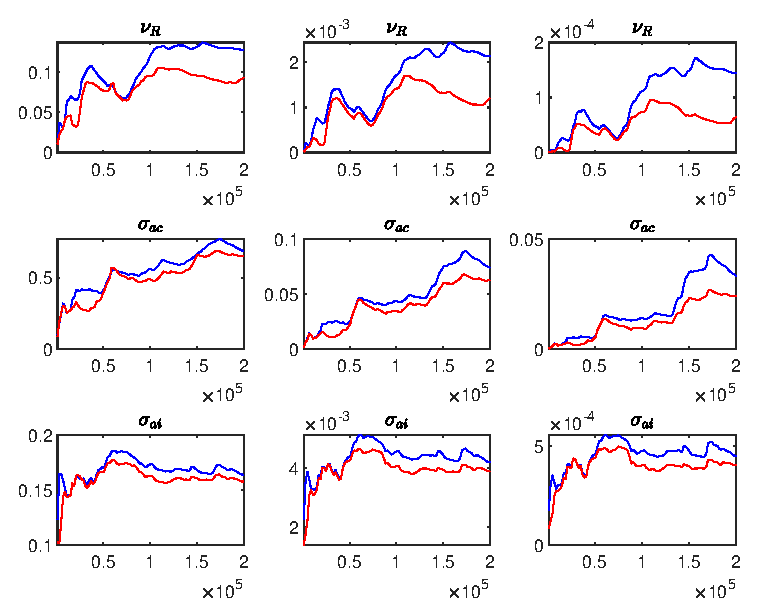
\includegraphics[width=0.80\textwidth]{BRS_sectoral_artificial_data/Output/BRS_sectoral_artificial_data_udiag6}
\caption{Univariate convergence diagnostics for the Metropolis-Hastings.
The first, second and third columns are respectively the criteria based on
the eighty percent interval, the second and third moments.}\label{Fig:UnivariateDiagnostics:6}
\end{figure}

\begin{figure}[H]
\centering 
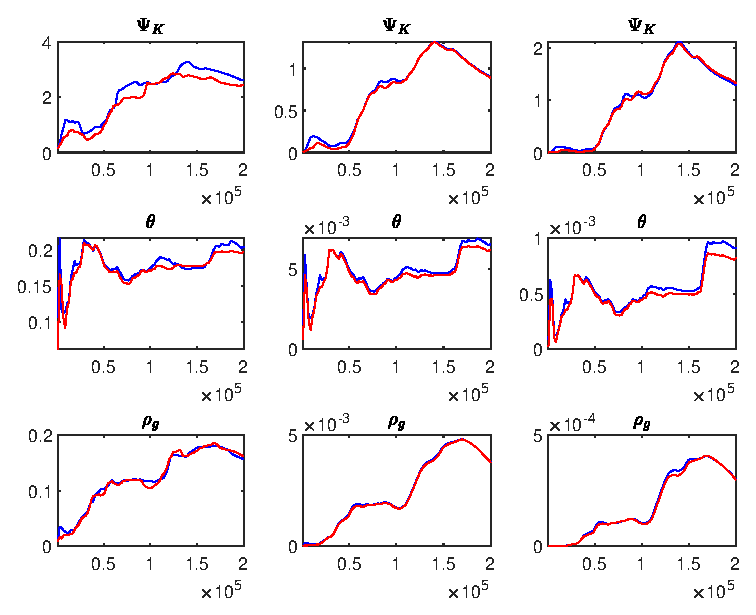
\includegraphics[width=0.80\textwidth]{BRS_sectoral_artificial_data/Output/BRS_sectoral_artificial_data_udiag7}
\caption{Univariate convergence diagnostics for the Metropolis-Hastings.
The first, second and third columns are respectively the criteria based on
the eighty percent interval, the second and third moments.}\label{Fig:UnivariateDiagnostics:7}
\end{figure}

\begin{figure}[H]
\centering 
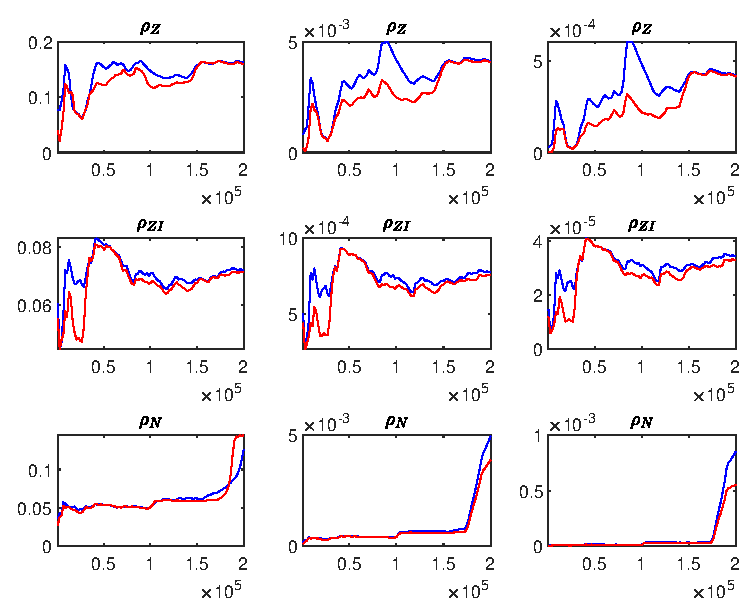
\includegraphics[width=0.80\textwidth]{BRS_sectoral_artificial_data/Output/BRS_sectoral_artificial_data_udiag8}
\caption{Univariate convergence diagnostics for the Metropolis-Hastings.
The first, second and third columns are respectively the criteria based on
the eighty percent interval, the second and third moments.}\label{Fig:UnivariateDiagnostics:8}
\end{figure}

\begin{figure}[H]
\centering 
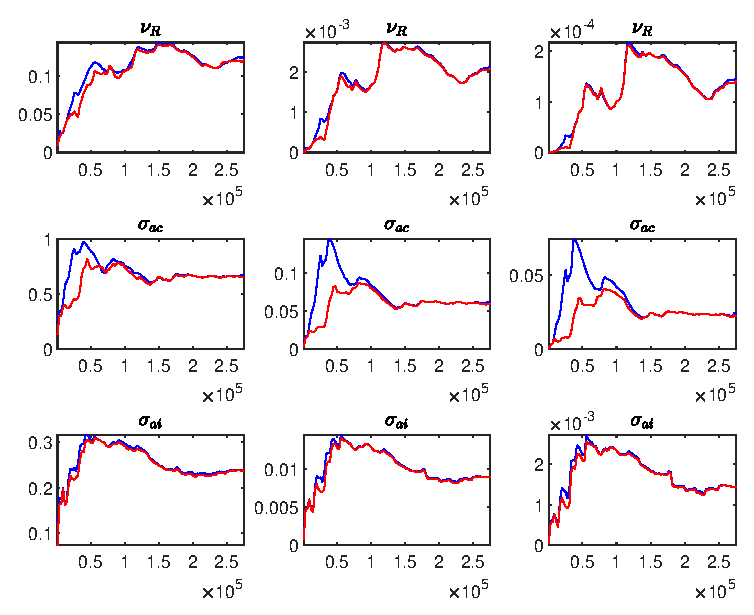
\includegraphics[width=0.80\textwidth]{BRS_sectoral_artificial_data/Output/BRS_sectoral_artificial_data_udiag9}
\caption{Univariate convergence diagnostics for the Metropolis-Hastings.
The first, second and third columns are respectively the criteria based on
the eighty percent interval, the second and third moments.}\label{Fig:UnivariateDiagnostics:9}
\end{figure}

\begin{figure}[H]
\centering 
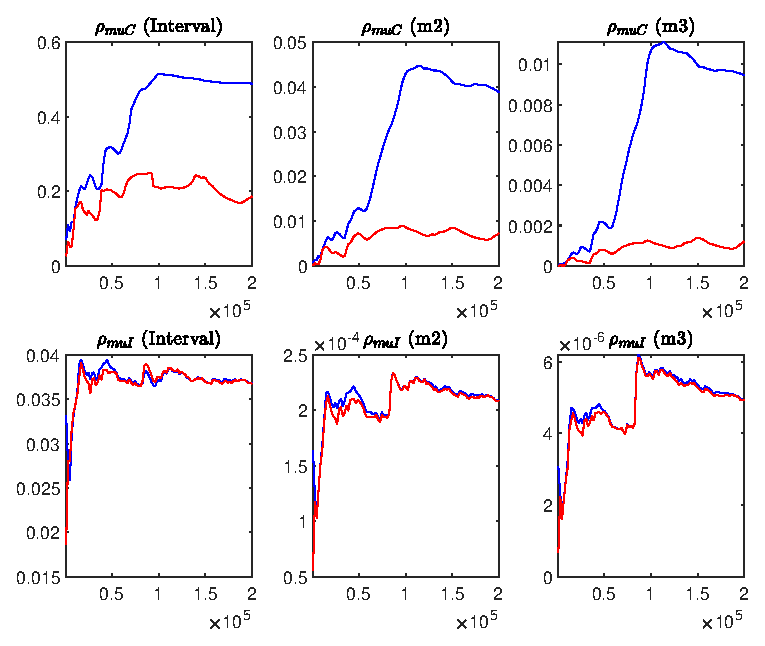
\includegraphics[width=0.80\textwidth]{BRS_sectoral_artificial_data/Output/BRS_sectoral_artificial_data_udiag10}
\caption{Univariate convergence diagnostics for the Metropolis-Hastings.
The first, second and third columns are respectively the criteria based on
the eighty percent interval, the second and third moments.}\label{Fig:UnivariateDiagnostics:10}
\end{figure}

\begin{figure}[H]
\centering 
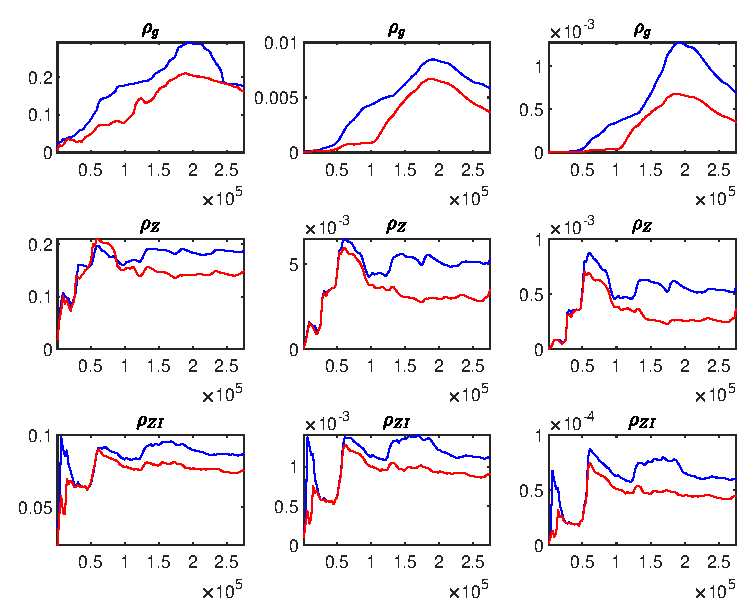
\includegraphics[width=0.80\textwidth]{BRS_sectoral_artificial_data/Output/BRS_sectoral_artificial_data_udiag11}
\caption{Univariate convergence diagnostics for the Metropolis-Hastings.
The first, second and third columns are respectively the criteria based on
the eighty percent interval, the second and third moments.}\label{Fig:UnivariateDiagnostics:11}
\end{figure}

\begin{figure}[H]
\centering 
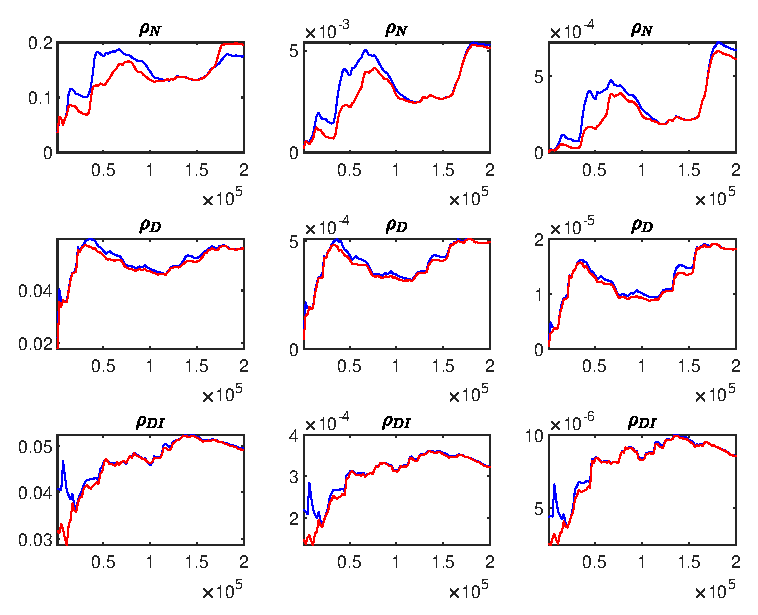
\includegraphics[width=0.80\textwidth]{BRS_sectoral_artificial_data/Output/BRS_sectoral_artificial_data_udiag12}
\caption{Univariate convergence diagnostics for the Metropolis-Hastings.
The first, second and third columns are respectively the criteria based on
the eighty percent interval, the second and third moments.}\label{Fig:UnivariateDiagnostics:12}
\end{figure}

\begin{figure}[H]
\centering 
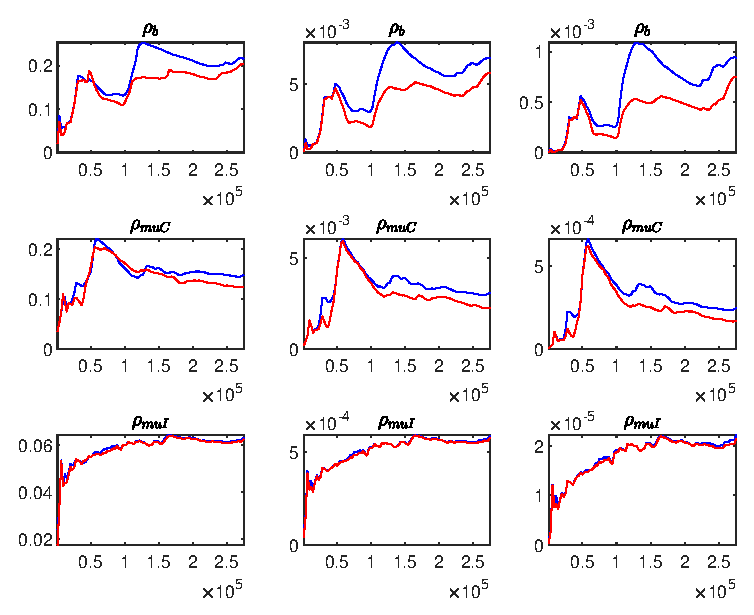
\includegraphics[width=0.80\textwidth]{BRS_sectoral_artificial_data/Output/BRS_sectoral_artificial_data_udiag13}
\caption{Univariate convergence diagnostics for the Metropolis-Hastings.
The first, second and third columns are respectively the criteria based on
the eighty percent interval, the second and third moments.}\label{Fig:UnivariateDiagnostics:13}
\end{figure}

